\section{CKAN}
\label{sec:ckan-webapp}

As said in Chapter \ref{chp:rdf-builder}, the \ac{RDF} Graph Builder get the data from three different sources, and one of these sources is the CKAN Open Data Portal of the city (Comune di Sona in this case). The main idea is to use this open source portal in order to facilitate the publication of data on the web and be aligned with other Italian and foreign cities. At the same time, this portal provides the catalog  compliant with the \verb#DCAT-AP_IT# metadata profile, and this allows published data to be made available in regional, national and European portals as well. In addition, the presence of data in \acl{LOD} format does not preclude the use of the CKAN portal, despite the fact that the latter's data achieve a three-star rating according to Tim Berners-Lee's classification introduced in Section \ref{sec:lod-stars}. In fact, in addition to having a lower management cost \cite{bauer2011linked}, this portal allows the publication of data that in \acl{LOD} format would not be publishable, or for which an ontology describing them has not yet been developed. It also allows original resources to be reused for other tasks, either by the municipality or by companies or citizens.

\paragraph*{}
The entire project is available under an open source license on GitHub at the link \url{https://github.com/luca-martinelli-09/ckan}. The final result built for the Comune di Sona is shown in Figure \ref{fig:ckan-sona}. For ease of installation and deployment, moreover, the portal has been containerized to produce a Docker\footnote{\url{https://www.docker.com/}} image.

\begin{figure}[!ht]
  \centering
  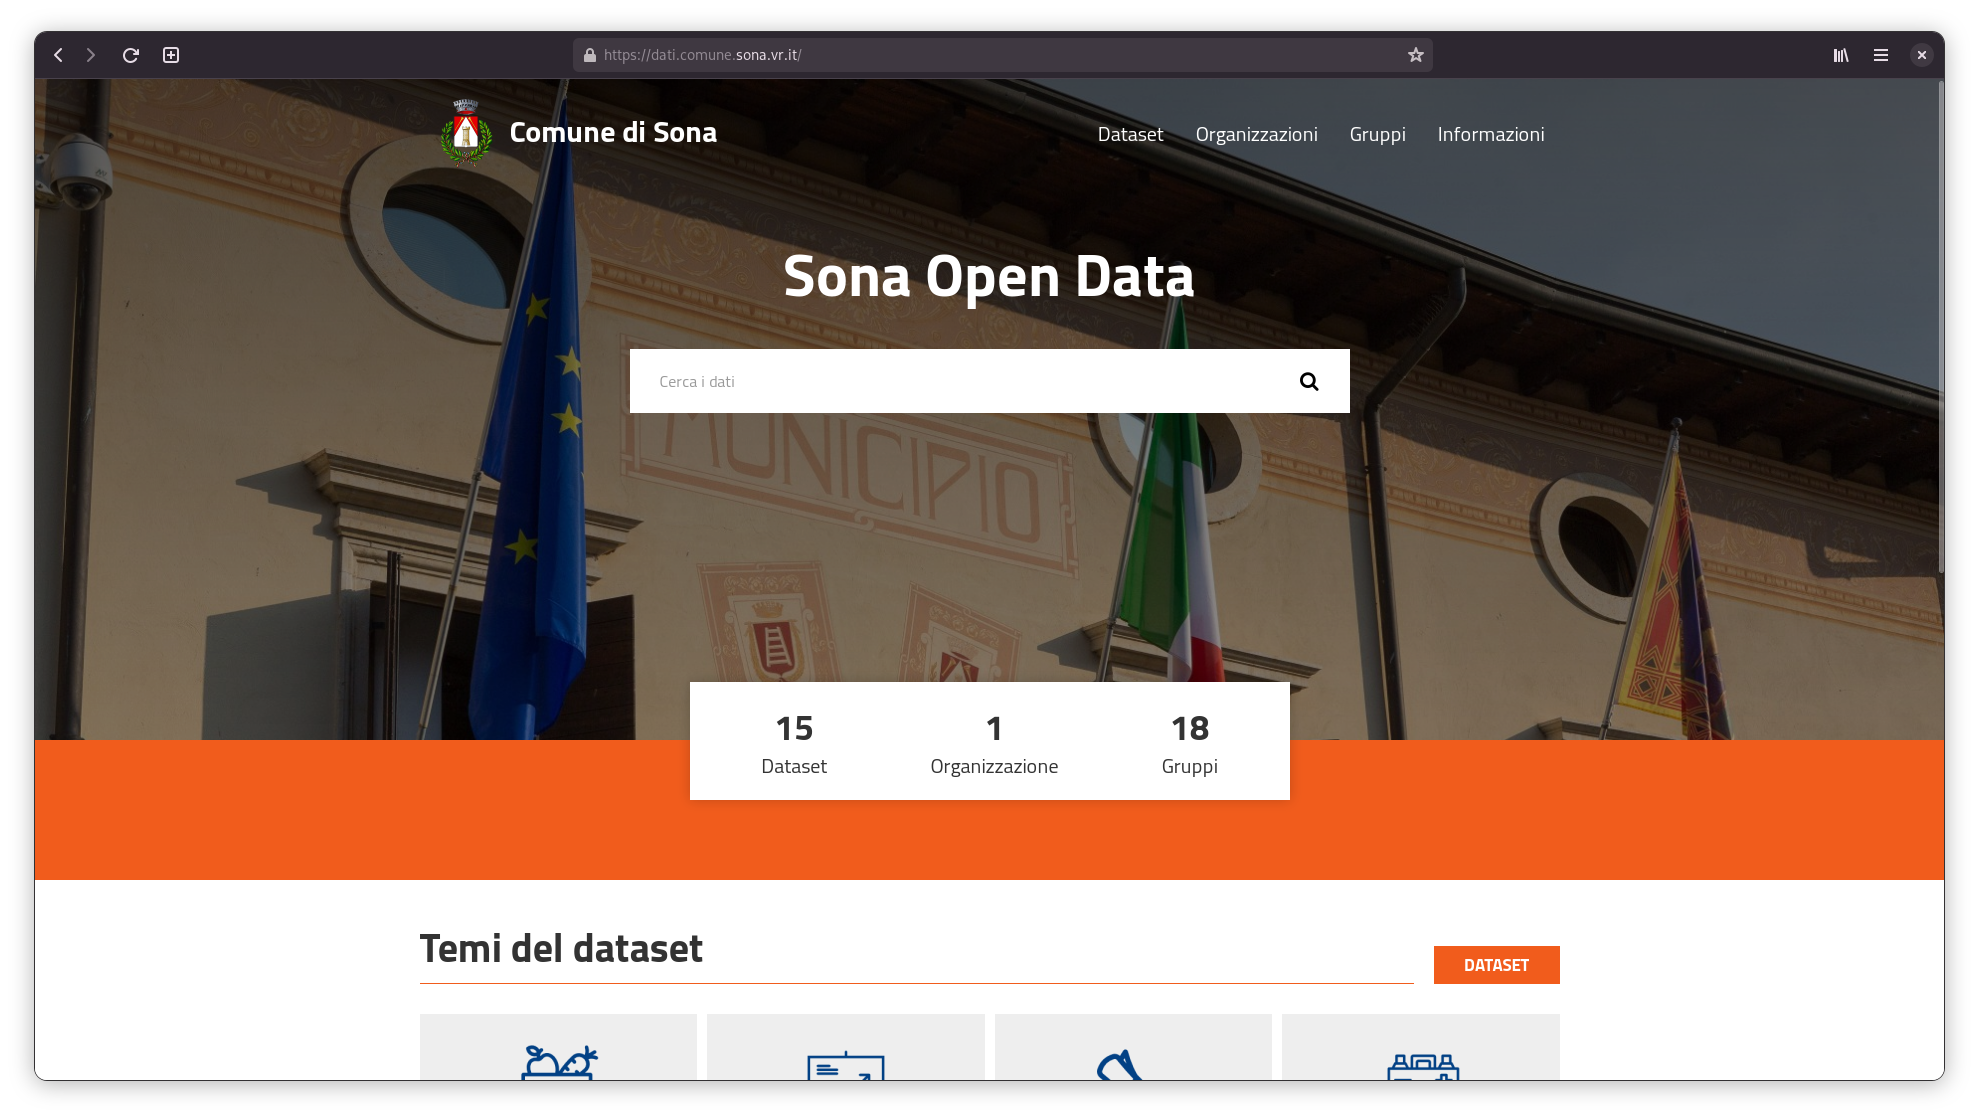
\includegraphics[width=\columnwidth]{images/ckan/ckan-sona}
  \caption{A snapshot of the Comune di Sona's CKAN Open Data portal.}
  \label{fig:ckan-sona}
\end{figure}

\paragraph*{}
The Open Data portal extends the CKAN 2.9 Docker image provided by the Open Knowledge Foundation,\footnote{\url{https://github.com/okfn/docker-ckan}} installing the required plugins. Such plugins are:

\begin{description}
  \item[View, DataStore, and DataPusher] These are the default plugins provided by CKAN. The View plugin is used to show a preview of the resources in form of tables or images. DataStore and DataPusher are two plugins that process \ac{CSV} files and enable the ability to use \acsp{API} to access data in \ac{JSON} format. Thanks to these plugins, it is also possible to filter data using the \acs{SQL} language;
  \item[Spatial] This plugin adds geospatial capabilities to CKAN, adding a spatial field to the dataset schema;
  \item[GeoView] This extension is used together with the spatial plugin, and contains view plugins to display geospatial files in CKAN;
  \item[Harvest] It provides a harvesting framework that allows data and catalogs to be imported from external \acsp{API}, \verb#DCAT# catalogs, or other CKAN portals;
  \item[Multilang] This extension provides a way to localize the CKAN's title and description contents for Dataset, Resources, Tags, Organizations, and Groups;
  \item[DCAT and DCAT-AP\_IT] These two plugins expose the data catalog as \ac{RDF} document serialized using the \verb#DCAT# and \verb#DCAT-AP_IT# profiles.
\end{description}

To further simplify the process of setting up the portal, there is a \verb#.env# configuration file that allows the main portal information to be specified, such as the account and password and administrator, the name, description and logo of the site, the email and vat number of the public administration that manages the portal, and a possible configuration of the email server for sending notifications. Code \ref{code:ckan-portal-env} shows the configuration template file.

\begin{lstlisting}[language=bash,caption={Configuration template file for the CKAN Open Data portal.},label=code:ckan-portal-env]
CKAN_SITE_URL # URL of the custom CKAN's portal

CKAN_SYSADMIN_NAME # Name of the sysadmin account
CKAN_SYSADMIN_PASSWORD # Password for the sysadmin account
CKAN_SYSADMIN_EMAIL # Email for the sysadmin account

CKAN_ORG_VAT # IPA/VAT/IVA of the organization
CKAN_ORG_EMAIL # Email of the organization

CKAN__DATAPUSHER__CALLBACK_URL_BASE # Same as CKAN_SITE_URL

# Core
CKAN__SITE_TITLE # The website title (usually the P.A. name)
CKAN__SITE_DESCRIPTION # Website description
CKAN__SITE_ABOUT # Website long description
CKAN__SITE_LOGO # Url for the logo
CKAN__FAVICON # Url for the favicon

# Email setup
CKAN_SMTP_SERVER
CKAN_SMTP_STARTTLS
CKAN_SMTP_USER
CKAN_SMTP_PASSWORD
CKAN_SMTP_MAIL_FROM

CKANEXT__DCAT__BASE_URI # Same as CKAN_SITE_URL

GEONAMES__USERNAME # Follow the guide for geosolutions-it/ckanext-dcatapit extension
\end{lstlisting}

Finally, a theme was developed for CKAN, which is installed on par with an extension, to apply graphical customization to the portal. The theme is also available under an open source license on GitHub at \url{https://github.com/luca-martinelli-09/ckanext-cdstheme/}.